\chapter{Implementation}
\label{ch:implementation}
This chapter focuses in detail on the technical implementation of the crowd/volunteer computing platform. Section \ref{sec:implementation:backend} and \ref{sec:implementation:frontend} briefly describe the usage of the platform and serve as documentation for this project.

\section{Architecture}
\label{sec:implementation:architecture}
The platform is divided into three components: the Backend or Server \ref{sec:implementation:backend}, the Frontend providing the web application for all Clients \ref{sec:implementation:frontend}, and a database.

\begin{figure}[htbp]
    \centering
    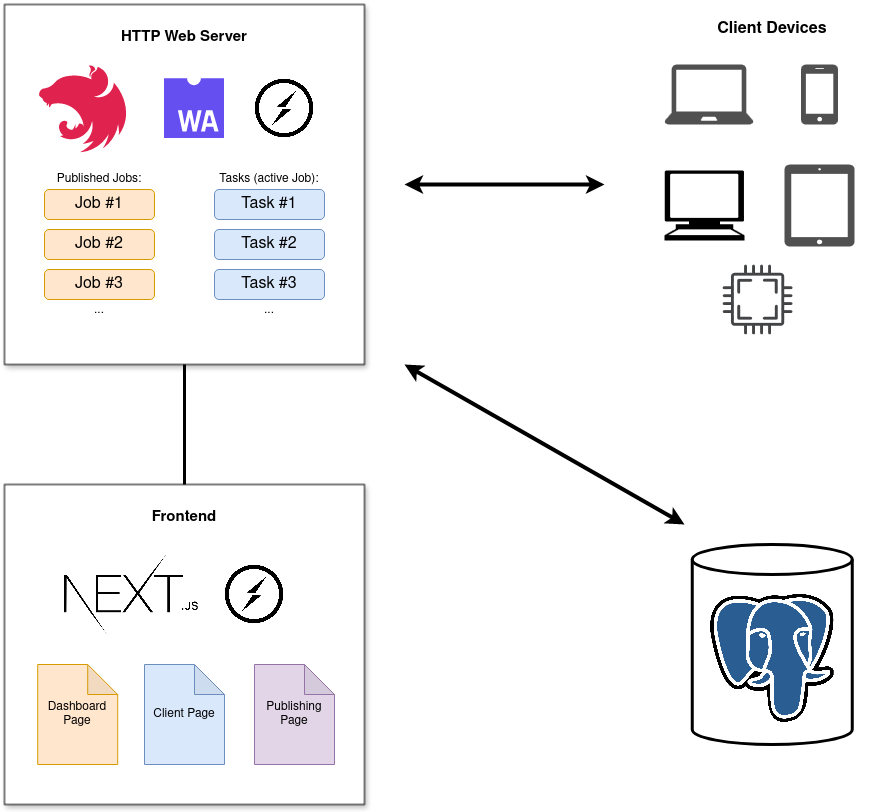
\includegraphics[width=0.95\textwidth]{gfx/figures/WebAssembly-MA.drawio.png}
    \caption{Architecture (Draft)}
    \label{fig:implementation:architecture}
\end{figure}

Figure \ref{fig:implementation:architecture} illustrates the architecture of the platform. Heterogenous clients, diverse in hardware or operating system, are able to connect to the platform. Each client (Worker and Administrator) is bidirectionally connected to the server through a WebSocket connection. The database is only accessible by the server.

\subsection{Communication}
\label{subsec:implementation:architecture:communication}
When clients establish a connection to the platform by accessing the frontend application, a WebSocket connection is initiated. This enables real-time and bidirectional communication between the Server and client. Therefore this connection is used to send Tasks from the Server to the Workers as well to send the result of each Tasks from the Worker to the Server. Furthermore, Administrators receive real-time data about all connected Workers and the current status of each Job through this WebSocket connection.

\begin{figure}[htbp]
    \centering
    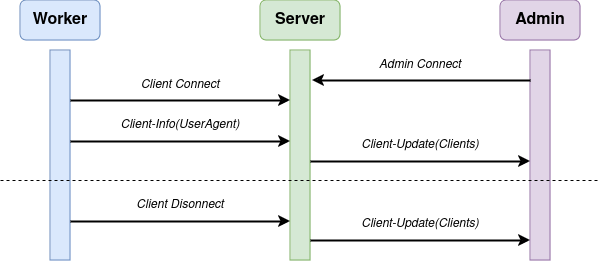
\includegraphics[width=0.95\textwidth]{gfx/figures/communication-connection.png}
    \caption{Communication: Connection of Worker \& real-time Update for Administrator}
    \label{fig:implementation:communication1}
\end{figure}

Figure \ref{fig:implementation:communication1} illustrates the process of a Worker connecting to the Server. Upon successful connection, the Worker transmits all available information regarding its hardware and operating system in form of the Browser User Agent to the Server. After this initialization of the Worker, all previously connected Administrators automatically receive an updated List of connected Workers. Similarly, if a Worker disconnects a automatic update is send to all Administrators.

\begin{figure}[htbp]
    \centering
    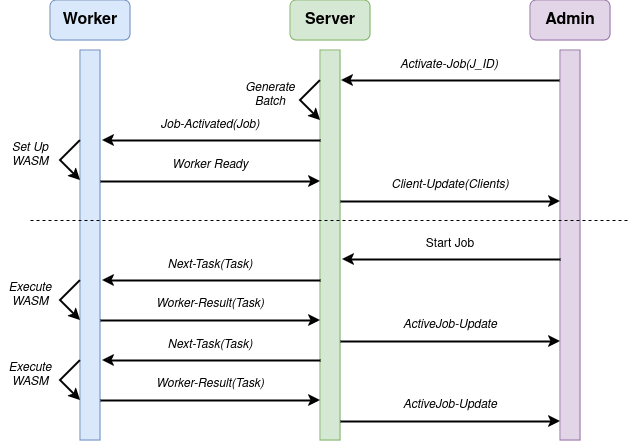
\includegraphics[width=0.95\textwidth]{gfx/figures/communication-jobexecution.png}
    \caption{Communication: Administrator starts Job \& Worker execute Tasks}
    \label{fig:implementation:communication2}
\end{figure}

Figure \ref{fig:implementation:communication2} illustrates the Job initiation and execution process. The sequence begins when an Administrator changes a Jobs status to \emph{ACTIVE}. The Server then generates a Batch of Tasks for the specified Job and notifies all connected Workers by transmitting the activated Job to them. Upon receiving this notification, each Worker retrieves the corresponding WebAssembly binary from the Server and initializes a WebWorker with the WebAssembly environment for this active Job. When this step is successfully completed the Worker notifies the Server which updates the Workers \emph{ready} attribute. This update is also forwarded to all Administrators.

If a Administrator changes the status of a active Job to \emph{RUNNING}, the Server than distributes unique tasks from the current batch to all workers that have transmitted the \emph{Worker Ready} message. Each worker executes its assigned Task, appends the result to the Task object, and transmits the completed Task back to the server. If unprocessed or unscheduled Tasks remain in the Batch, the Server responds by assigning the next pending Task to the Worker. Additionaly, the Server notifies all Administrators of each successfully completed Task.

If a Worker is connecting while there is a active or running Job, the communication sequence is executed identically. This enables dynamic participation in ongoing Jobs for Workers.

\begin{figure}[htbp]
    \centering
    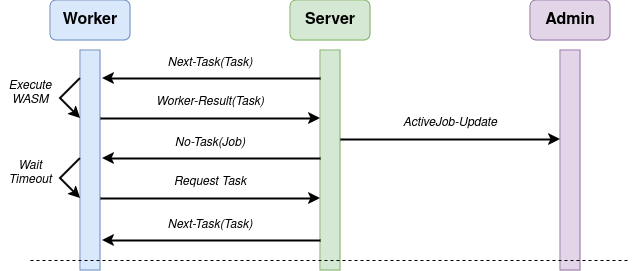
\includegraphics[width=0.95\textwidth]{gfx/figures/communication-timeout.png}
    \caption{Communication: Administrator starts Job \& Worker execute Tasks}
    \label{fig:implementation:communication3}
\end{figure}

Each Job has a timeout attribute for its Tasks. Scheduled Tasks that remain incomplete after their allocated timeout period can be redistributed to a different Worker. This mechanism enables the rescheduling of Tasks, which have been assigned to a malfunctioning Worker or a Worker that has disconnected before completing its assigned Task. Additionally, the system allows rescheduling of Tasks that have been assigned to slower Workers, known as Stragglers, to more efficient Workers. Hence this mechanism can optimize the overall execution time of a Job.

Figure \ref{fig:implementation:communication3} illustrates the case, if all Tasks of the Batch already have been scheduled, but one or more are not yet completed. When a Worker transmits a completed Task to the Server while the timeout period of all other scheduled Tasks has not expired, the Server responds with the \emph{No-Task} message accompanied by the Job object of the currently active Job. The Worker extracts the timeout value from this Job objects and initiates a waiting period equivalent to the timeout value plus a randomized overhead. This additional randomized overhead time prevents simultaneous Task requests from multiple Workers. After the completion of the waiting period, the Worker transmits a \emph{Request Task} message to the Server. The server responds either with a newly available Task or another \emph{No-Task} message, repeating this sequence until the current batch is fully processed.

\subsection{Persistence}
\label{subsec:implementation:architecture:persistence}


\subsubsection{Database}

\subsubsection{Task Input and Task Result}

\subsection{Scheduling}
\label{subsec:implementation:architecture:scheduling}


\section{Backend}
\label{sec:implementation:backend}
API endpoints 

\section{Frontend}
\label{sec:implementation:frontend}
Design and UI / Pages

\section{Security through Authentication}
\label{sec:implementation:authentication}
How can meliccious use can be prevented?

what is a JWT ? How is JWT used in this project? User vs Admin JWT

\section{Challenges}
\label{sec:implementation:challenges}
what was difficult?
\begin{itemize}
    \item Hadel Input and Output
    \item Output as File (PNG)
    \item Prevent dublicate Task execution
    \item Minimize Communication
\end{itemize}